% !TEX program = xelatex
% !TEX encoding = UTF-8 Unicode
\documentclass[13pt,a4paper,oneside]{report}

\usepackage{fontspec}
\usepackage{polyglossia}
\setmainlanguage{english}
\setotherlanguage{vietnamese}
\setmainfont{lmroman10-regular.otf}[
  BoldFont=lmroman10-bold.otf,
  ItalicFont=lmroman10-italic.otf,
  BoldItalicFont=lmroman10-bolditalic.otf]
\usepackage{geometry}
\geometry{a4paper,left=3cm,right=2cm,top=2cm,bottom=2cm}
\usepackage{setspace}
\onehalfspacing
\usepackage{amsmath,amssymb}
\usepackage{graphicx}
\usepackage{booktabs}
\usepackage{tabularx}
\usepackage{float}
\usepackage{caption}
\usepackage{siunitx}
\sisetup{group-separator={,},group-minimum-digits=4,detect-all}
\captionsetup{font=small,labelfont=bf,labelsep=endash}
\usepackage[table]{xcolor}
\usepackage{tikz}
\usetikzlibrary{arrows.meta,positioning,fit,backgrounds}
\usepackage[unicode,hidelinks]{hyperref}

\urlstyle{tt}
\def\UrlBreaks{\do\/\do\_\do\.\do\-\do\,\do\{\do\}}
\Urlmuskip=0mu plus 1mu\relax

\usepackage{titlesec}
\titleformat{\chapter}[display]
  {\normalfont\Large\bfseries\centering}{\chaptertitlename\ \thechapter}{12pt}{\LARGE}
\titlespacing*{\chapter}{0pt}{10pt}{24pt}
\setlength{\parindent}{1.2em}
\setlength{\emergencystretch}{3em}

\begin{document}
\sloppy

\begin{titlepage}
\centering
{\large MINISTRY OF EDUCATION AND TRAINING\par}
{\large FPT SCHOOL OF BUSINESS \& TECHNOLOGY (FSB), FPT UNIVERSITY\par}
\vfill
{\LARGE\bfseries REPRODUCTION AND CONTROLLED EVALUATION OF CRYPTOMAMBA\\[6pt]
FOR NEXT-DAY BITCOIN PRICE FORECASTING\par}
\vspace{10pt}
{\large MASTER'S THESIS\par}
\vfill
\begin{flushright}
\begin{tabular}{@{}ll@{}}
Student: & Trần Huỳnh Anh Hiếu \\
Supervisor: & Nguyễn Duy Nghiêm \\
\end{tabular}
\end{flushright}
\vfill
{\large Vietnam --- 2026\par}
\end{titlepage}

\pagenumbering{roman}

\chapter*{Abstract}
\addcontentsline{toc}{chapter}{Abstract}
This thesis reproduces CryptoMamba-v (CM-v) for next-day Bitcoin closing-price forecasting and
reassesses the original paper's findings. Under the 350-day protocol, the reproduced checkpoint's
RMSE, MAE, and MAPE differ from the reported values by \num{0.892}\%, \num{1.057}\%, and
\num{0.718}\%, respectively. The controlled evaluation then compares CM-v, the experimental
CMamba-T/S5-Full model, and naive persistence on the same 304 validation dates and 304 test dates.
Their test RMSE values are \num{1703.51}, \num{1660.83}, and \num{1657.55}. Neither the
Diebold--Mariano test nor the block-bootstrap interval confirms an RMSE advantage for S5-Full over
CM-v. CM-v reaches \num{57.57}\% directional accuracy, but McNemar's test does not confirm a
directional difference between the two models. Persistence is excluded from this metric because it
carries the current price forward.
The paired RMSE and directional conclusions remain unchanged for bootstrap block lengths
$L=\num{5},\num{7},\num{14}$.

Two additional evaluation layers are provided. First, a zero-cost replay preserves the paper's
released trading algorithms for checkpoint reconciliation. Second, a separate self-financing
engine charges transaction costs on traded notional, limits gross exposure, and reconciles final
equity. Buy-and-hold exceeds every forecast-driven strategy at all three costs; at a \num{0.2}\%
test cost, it ends at \$\num{158.09}. S5-Full has \num{57249} parameters compared with
\num{136952} for CM-v.
It achieves lower RMSE than CM-v on validation and test, but does not outperform persistence.
Finally, a five-screen Console presents data, evaluation, checkpoint inference, trading, and
architecture. Its primary workflow accepts a new dataset, selects either the CM-v or S5-Full
checkpoint, and produces a forecast without retraining.

The application context is Vietnam's pilot crypto-asset market under Resolution
05/2025/NQ-CP. The thesis does not provide legal analysis or investment advice.

\vspace{6pt}
\noindent\textbf{Keywords:} \textit{Bitcoin, time-series forecasting, Mamba, research
reproduction, naive persistence, forecast testing, self-financing backtest, Vietnamese crypto-asset
market.}

\tableofcontents
\listoffigures
\addcontentsline{toc}{chapter}{List of Figures}
\listoftables
\addcontentsline{toc}{chapter}{List of Tables}

\chapter*{List of Abbreviations}
\addcontentsline{toc}{chapter}{List of Abbreviations}
\renewcommand{\arraystretch}{1.22}
\begin{tabularx}{\linewidth}{@{}lX@{}}
\toprule
\textbf{Abbreviation} & \textbf{Meaning} \\
\midrule
API & Application Programming Interface \\
BTC & Bitcoin \\
CM-v & CryptoMamba-v, the variant that includes volume \\
DM & Diebold--Mariano \\
HAC & Heteroskedasticity and Autocorrelation Consistent \\
MAE & Mean Absolute Error \\
MAPE & Mean Absolute Percentage Error \\
MDD & Maximum Drawdown \\
OHLCV & Open--High--Low--Close--Volume \\
RMSE & Root Mean Square Error \\
ROI & Return on Investment \\
SSM & State Space Model \\
\bottomrule
\end{tabularx}
\renewcommand{\arraystretch}{1.0}

\cleardoublepage
\pagenumbering{arabic}

% ---------------------------------------------------------------------
\chapter{Introduction}\label{chap:intro}

\section{Research Context}\label{sec:motivation}
Next-day Bitcoin price forecasting is difficult because the price series is non-stationary, highly
volatile, and strongly autocorrelated at the absolute-price scale. In this setting, a low error
alone does not demonstrate that a model extracts new information: simply carrying the current
closing price forward is already a strong control.

The CryptoMamba paper \cite{cryptomamba} applies Mamba \cite{mamba} to daily BTC-USD data and
reports that CryptoMamba-v outperforms LSTM-v, Bi-LSTM-v, GRU-v, iTransformer-v, and S-Mamba-v in
RMSE, MAE, and MAPE. It also feeds forecasts into three trading algorithms. However, the published
tables contain only aggregate metrics, without date-level errors for paired tests, and the trading
evaluation does not model transaction costs through a self-financing ledger. This thesis addresses
that evaluation gap while also implementing a lightweight variant and an inspectable explanatory
system.

\section{Objectives and Research Questions}\label{sec:rq}
The objective is to reproduce CM-v, evaluate forecasting and trading under defined protocols,
experiment with a lightweight variant, and visualize the full workflow in a five-screen Console.
The four research questions are:
\begin{itemize}
\item \textbf{RQ1 -- Reproduction.} To what extent do CM-v and the released trading replay reproduce
the paper's results?
\item \textbf{RQ2 -- Evaluation.} On identical target dates, how do CM-v, S5-Full, and naive
persistence differ in forecast error, direction, and statistical significance?
\item \textbf{RQ3 -- Trading.} How do forecast results translate into trading outcomes when the
paper replay is separated from a corrected self-financing engine with costs?
\item \textbf{RQ4 -- Model.} Does S5-Full provide a lighter model with sufficient experimental
evidence to support a forecasting advantage?
\end{itemize}

\section{Scope}\label{sec:scope}
The study uses one asset, BTC-USD, with daily OHLCV candles, a one-step forecast horizon, and the
time periods defined by the paper. The local controlled evaluation includes only three models with
date-level predictions that can be aligned exactly: reproduced CM-v, S5-Full, and naive
persistence. Other model rows appear only in the \emph{Paper-reported} reference table and are not
included in local paired tests.

As an application context, the project is situated within Vietnam's five-year pilot crypto-asset
market under Resolution 05/2025/NQ-CP, effective from 09-09-2025 \cite{nq05}. The Resolution
defines context only; the technical scope does not extend to legal analysis, compliance
assessment, or investment advice.

The primary workflow is paper data or a new CSV $\to$ data validation $\to$ CM-v/S5-Full
checkpoint selection $\to$ next-day price prediction. Historical replay is retained to illustrate
past behavior. External HTTP inference is optional rather than a prerequisite. The product is a
research prototype, not an advisory or trade-execution system.

\section{Contributions}\label{sec:contrib}
\begin{enumerate}
\item \textbf{Reproduction.} Reproduce CM-v, reconcile the official and reproduced checkpoints, and
audit the paper's trading replay.
\item \textbf{Evaluation.} Add naive persistence, compare models on identical target dates, and test
the observed differences using DM and Wilcoxon procedures.
Uncertainty, chronological variation, and fee sensitivity are evaluated using block bootstrap,
chronological halves, and three fixed fee rates.
\item \textbf{Model.} Implement and evaluate S5-Full as a lightweight CMamba-T experiment, reporting
positive, negative, and non-significant results on their correct splits.
\item \textbf{System.} Build a five-screen Console for the
data $\to$ prediction $\to$ evaluation $\to$ trading $\to$ architecture flow, with direct
inference from two local checkpoints.
\end{enumerate}

% ---------------------------------------------------------------------
\chapter{Background and Related Work}\label{chap:background}

\section{Time-Series Forecasting and the Persistence Baseline}\label{sec:persistence}
For one-step forecasting, naive persistence is defined as
\begin{equation}\label{eq:persistence}
\widehat{y}_{t+1}=y_t,
\end{equation}
where $y_t$ is the current closing price. This baseline has no trainable parameters and issues
neither upward nor downward signals. It tests whether a deep model improves on the most recent
observation or merely reproduces the current price level.

iTransformer reverses the conventional Transformer tokenization scheme to model relationships
across variables \cite{itransformer}. S-Mamba uses bidirectional Mamba for cross-variable
relationships and a feed-forward network for temporal relationships \cite{smamba}. Both
architectures appear in CryptoMamba's comparison table, but this thesis uses only their published
aggregate metrics because date-level forecasts are unavailable.

\section{State Space Models and Mamba}\label{sec:mamba}
A linear SSM represents hidden state $h_t$ and output $z_t$ as
\begin{equation}\label{eq:ssm}
h_t=\bar{A}h_{t-1}+\bar{B}x_t, \qquad z_t=Ch_t.
\end{equation}
Mamba makes state-transition parameters input-dependent, allowing information to be retained or
discarded at each sequence element while maintaining linear complexity in sequence length
\cite{mamba}. The interpretation of a scan therefore depends directly on which tensor axis is
treated as the sequence axis.

\section{CryptoMamba-v: Published Description and Released Execution Path}\label{sec:cmv}
The paper describes CryptoMamba as a sequence of C-Blocks followed by a Merge block. Each C-Block
contains multiple CMBlocks and an MLP; the input is a window of past observations and the output is
the next-day closing price \cite{cryptomamba}. Figure~\ref{fig:paper-source-architecture}
separates this conceptual description from behavior that can be verified in the released source.

\begin{figure}[H]
\centering
\resizebox{\linewidth}{!}{% Paper description versus the released CM-v execution path.
\begingroup
\definecolor{archBlue}{HTML}{E8F0FB}
\definecolor{archBlueEdge}{HTML}{5A7FBE}
\definecolor{archGreen}{HTML}{E4F3EC}
\definecolor{archGreenEdge}{HTML}{418B72}
\definecolor{archGold}{HTML}{FFF1CF}
\definecolor{archGoldEdge}{HTML}{B4882C}
\definecolor{archGrey}{HTML}{F5F7F9}
\definecolor{archGreyEdge}{HTML}{AAB4BD}
\definecolor{archInk}{HTML}{263238}

\tikzset{
  input/.style={draw=archBlueEdge, fill=archBlue, rounded corners=3pt,
    minimum width=2.9cm, minimum height=1.05cm, align=center, inner sep=4pt,
    font=\sffamily\small\bfseries, text=archInk},
  process/.style={draw=archGreenEdge, fill=archGreen, rounded corners=3pt,
    minimum width=2.6cm, minimum height=1.05cm, align=center, inner sep=4pt,
    font=\sffamily\small\bfseries, text=archInk},
  repeat/.style={draw=archGreenEdge, fill=archGreen, rounded corners=3pt,
    minimum width=1.75cm, minimum height=1.05cm, align=center, inner sep=3pt,
    font=\sffamily\small\bfseries, text=archInk},
  stage/.style={repeat, minimum width=2.45cm, minimum height=1.30cm},
  head/.style={draw=archGoldEdge, fill=archGold, rounded corners=3pt,
    minimum width=2.25cm, minimum height=1.05cm, align=center, inner sep=4pt,
    font=\sffamily\small\bfseries, text=archInk},
  output/.style={draw=archBlueEdge, fill=archBlue, rounded corners=3pt,
    minimum width=2.2cm, minimum height=1.05cm, align=center, inner sep=4pt,
    font=\sffamily\small\bfseries, text=archInk},
  group/.style={draw=archGreenEdge, fill=archGreen!38, dashed, rounded corners=5pt,
    line width=0.75pt, inner xsep=5pt, inner ysep=5pt},
  lane/.style={draw=archGreyEdge, fill=archGrey, rounded corners=6pt,
    line width=0.65pt, inner xsep=7pt, inner ysep=8pt},
  note/.style={font=\sffamily\scriptsize, text=archInk, align=center},
  title/.style={font=\sffamily\small\bfseries, text=archInk, align=left},
  flow/.style={-{Stealth[scale=1.2]}, draw=archInk, line width=0.85pt}
}

\begin{tikzpicture}[font=\sffamily\small, node distance=0.6cm and 0.8cm]
  \node[input] (paperInput)
    {14-day input\\{\scriptsize\mdseries OHLCV + Timestamp}};
  \node[repeat, right=of paperInput] (paperBlockOne)
    {C-Block 1};
  \node[repeat, right=of paperBlockOne] (paperBlockTwo)
    {C-Block 2};
  \node[repeat, right=of paperBlockTwo] (paperBlockThree)
    {C-Block 3};
  \node[head, right=of paperBlockThree] (paperMerge)
    {Merge};
  \node[output, right=of paperMerge] (paperOutput)
    {Next Close};

  \node[note, above=0.18cm of paperBlockTwo] (paperGroupTitle)
    {C-Blocks};
  \node[title, above=0.34cm of paperInput.north west, anchor=south west] (paperTitle)
    {Paper description\\[-1pt]{\scriptsize\mdseries Sections 4.1--5.1 and Figure 1}};

  \draw[flow] (paperInput) -- (paperBlockOne);
  \draw[flow] (paperBlockOne) -- (paperBlockTwo);
  \draw[flow] (paperBlockTwo) -- (paperBlockThree);
  \draw[flow] (paperBlockThree) -- (paperMerge);
  \draw[flow] (paperMerge) -- (paperOutput);

  \node[input, below=3.0cm of paperInput] (sourceInput)
    {Tensor\\$[B,6,14]$};
  \node[stage, right=of sourceInput] (sourceStageOne)
    {Stage 1\\{\scriptsize\mdseries 4 CMBlocks}\\{\scriptsize\mdseries Linear 14 $\to$ 16}};
  \node[stage, right=of sourceStageOne] (sourceStageTwo)
    {Stage 2\\{\scriptsize\mdseries 4 CMBlocks}\\{\scriptsize\mdseries Linear 16 $\to$ 32}};
  \node[stage, right=of sourceStageTwo] (sourceStageThree)
    {Stage 3\\{\scriptsize\mdseries 4 CMBlocks}\\{\scriptsize\mdseries Linear 32 $\to$ 1}};
  \node[head, right=of sourceStageThree] (sourceHead)
    {Permute +\\{\scriptsize\mdseries Linear 6 $\to$ 1}};
  \node[output, right=of sourceHead] (sourceOutput)
    {Next Close};

  \node[note, above=0.18cm of sourceStageTwo] (sourceGroupTitle)
    {3 stages; scan over 6 feature tokens};
  \node[title, above=0.34cm of sourceInput.north west, anchor=south west] (sourceTitle)
    {Released implementation\\[-1pt]{\scriptsize\mdseries \texttt{CMamba.forward}}};

  \draw[flow] (sourceInput) -- (sourceStageOne);
  \draw[flow] (sourceStageOne) -- (sourceStageTwo);
  \draw[flow] (sourceStageTwo) -- (sourceStageThree);
  \draw[flow] (sourceStageThree) -- (sourceHead);
  \draw[flow] (sourceHead) -- (sourceOutput);

  \begin{scope}[on background layer]
    \node[lane,
      fit=(paperTitle)(paperInput)(paperBlockOne)(paperBlockThree)(paperMerge)(paperOutput)
          (paperGroupTitle)] {};
    \node[group, fit=(paperBlockOne)(paperBlockThree)(paperGroupTitle)] {};
    \node[lane,
      fit=(sourceTitle)(sourceInput)(sourceStageOne)(sourceStageThree)
          (sourceHead)(sourceOutput)(sourceGroupTitle)] {};
    \node[group, fit=(sourceStageOne)(sourceStageThree)(sourceGroupTitle)] {};
  \end{scope}
\end{tikzpicture}
\endgroup
}
\caption[Paper diagram and released CM-v execution]{Paper-described pipeline versus the
source-derived CM-v execution path. The upper row combines the data/input description in Sections
4.1 and 5.1 with the architecture in Section 4.2 and Figure 1 of CryptoMamba; the lower row is
derived from the released \texttt{CMamba.forward} implementation.}
\label{fig:paper-source-architecture}
\end{figure}

In the released code, CM-v accepts a $[B,6,14]$ tensor. The Mamba block receives six feature tokens,
each with width 14. Three linear stages change the width as $14\to16\to32\to1$, and each stage
contains four CMBlocks. The final head permutes the tensor and applies Linear $6\to1$. The
executable configuration has \num{136952} parameters. This observation describes only the released
execution path; the paper's conceptual diagram does not expose tensor-axis details.

\section{Forecast Accuracy Comparison}\label{sec:stats-background}
The Diebold--Mariano (DM) test evaluates the null hypothesis that two forecasts have equal
predictive accuracy \cite{dm}. This thesis uses the squared-loss differential
$d_t=e_{A,t}^{2}-e_{B,t}^{2}$ with a HAC variance estimate at lag 1 following Newey--West
\cite{neweywest}. The Wilcoxon signed-rank test \cite{wilcoxon} is applied independently to the
absolute-error differential $|e_{A,t}|-|e_{B,t}|$. These tests answer different questions and are
therefore not presented as interchangeable measurements.

% ---------------------------------------------------------------------
\chapter{Research Methodology}\label{chap:method}

\section{Data and Chronological Splits}\label{sec:data}
Daily BTC-USD data follow the paper's protocol from 17-09-2018 to 17-09-2024. Input fields are
Timestamp, Open, High, Low, Close, and Volume. Splits preserve chronological order without
shuffling (Table~\ref{tab:splits}).

\begin{table}[htbp]
\centering
\caption{Data splits under the CryptoMamba protocol.}
\label{tab:splits}
\begin{tabularx}{\linewidth}{@{}lXX@{}}
\toprule
\textbf{Split} & \textbf{Period} & \textbf{Role} \\
\midrule
Train & 17-09-2018 to before 17-09-2022 & Parameter estimation \\
Validation & 17-09-2022 to before 17-09-2023 & Checkpoint selection \\
Test & 17-09-2023 to before 17-09-2024 & Final evaluation \\
\bottomrule
\end{tabularx}
\end{table}

CM-v uses a 14-day window, whereas S5-Full uses a 60-day window. Paired comparisons use the
intersection of target dates for which all three models produce forecasts: 304 validation dates
from 16-11-2022 to 15-09-2023 and 304 test dates from 16-11-2023 to 14-09-2024. All local tables,
tests, and corrected backtests use these 304 common target dates. The 350-day aggregate under the
paper protocol is used only for RQ1 and is not mixed with the 304-day paired evaluation.

\section{Models and Checkpoints}\label{sec:model-contracts}
Both models are evaluated against the same final target: the raw next-day Close. Their input and
output contracts differ as summarized in Table~\ref{tab:model-contracts}.

\begin{table}[H]
\centering
\caption{CM-v and S5-Full input, preprocessing, and output contracts.}
\label{tab:model-contracts}
{\small
\begin{tabularx}{\linewidth}{@{}lXX@{}}
\toprule
\textbf{Component} & \textbf{CM-v} & \textbf{S5-Full} \\
\midrule
Final target & Raw next-day Close & Raw next-day Close \\
Input window & 14 days, $[B,6,14]$ & 60 days, $[B,5,60]$ \\
Input fields & Timestamp + OHLCV & OHLCV; no Timestamp \\
Price input & Raw prices & $x/C_t-1$ \\
Volume input & $\mathrm{Volume}/10^9$ & $\log(1+\mathrm{Volume}/10^9)$ \\
Model output & Next-day Close & Relative return $\widehat r_{t+1}$ \\
Final prediction & Direct output & $C_t(1+\widehat r_{t+1})$ \\
\bottomrule
\end{tabularx}}
\end{table}

The reproduced checkpoint is used for CM-v evaluation and local inference. S5-Full is the local
experiment identifier for the CMamba-T architecture; it is not the published S5 layer as an
independent SSM family. Four CMBlocks with $d_{state}=16$ process its 60 day-token sequence. The
latest-day representation passes through LayerNorm and Linear $32\to1$. The seed-23 checkpoint,
selected at best epoch 321, has \num{57249} parameters.

Both models are therefore scored in the same price space and on the same target dates. Because the
input window, preprocessing, output parameterization, and architecture change together, this is an
end-to-end model-pipeline comparison, not an architecture-only ablation.

For inference, the data are validated and the model-specific window is selected before loading the
chosen checkpoint. Prediction does not update the model weights.

\section{Metrics and Statistical Tests}\label{sec:metrics}
For $e_t=y_t-\widehat{y}_t$, the three primary metrics are
\begin{align}
\mathrm{RMSE} &= \sqrt{\frac{1}{n}\sum_{t=1}^{n}e_t^2}, &
\mathrm{MAE} &= \frac{1}{n}\sum_{t=1}^{n}|e_t|, \\
\mathrm{MAPE} &= \frac{100}{n}\sum_{t=1}^{n}\left|\frac{e_t}{y_t}\right|.
\end{align}
Forecast direction is the sign of $\widehat{y}_{t+1}-y_t$, and realized direction is the sign of
$y_{t+1}-y_t$. Directional accuracy is calculated only for models that produce an upward or
downward forecast; naive persistence is excluded from this metric. DM and Wilcoxon tests use the
exact paired dates, are two-sided, and use significance level $\alpha=0.05$.

To preserve serial dependence, the thesis uses a non-circular moving-block bootstrap
\cite{kunsch1989,buhlmann1999}. For $n=304$, it fixes
$L=\lceil n^{1/3}\rceil=\num{7}$ as an $n^{1/3}$-order heuristic, uses \num{50000} resamples, and
sets bootstrap computation seed \num{230813}, distinct from the training seed. The paired analysis
is repeated at $L=\num{5}$ and $L=\num{14}$ while the data, forecasts, resample count, and
computation seed remain fixed. Here $L$ denotes bootstrap block length, not the model input window.
$L=\num{7}$ is not claimed to be optimal. The percentile 95\%
intervals assume approximate stationarity and short-range dependence within each split; they do
not estimate retraining variation or uncertainty under future market regimes. Intervals are
reported for each model's RMSE, paired RMSE differences, and directional accuracy. An exact
McNemar test on paired correct/incorrect directional outcomes is supplementary
\cite{mcnemar1947}; the block-bootstrap interval is primary when accounting for serial dependence.

\section{Two Trading Protocols}\label{sec:trading-method}
\textbf{Paper replay} executes the released Vanilla, Smart, and Extended Smart algorithms with
initial capital of \$100 and zero fees. Its purpose is to audit reproduction of Table 4 in the
paper; it is not an economically corrected simulation.

\textbf{Corrected self-financing} is a separate engine. A signal at day $t$ uses only the current
Close and the forecast for Close $t+1$. Orders execute at the signal-day Close to preserve the
same-close convention, after which positions are marked at the target Close. Fees are charged on
absolute traded notional and included in position sizing. The engine maintains cash and BTC
positions, tracks short collateral, limits gross exposure to 1x, and verifies
\begin{equation}\label{eq:reconcile}
\mathrm{equity}_{\mathrm{final}}=
\mathrm{cash}_{T}+q_Tp_T,
\end{equation}
where transaction fees and borrow costs are deducted directly from cash before marking positions.
The result matrix uses transaction-cost rates of 0\%, 0.1\%, and 0.2\%; 0.2\% is the thesis
reporting reference. Borrow cost is set to zero in this experiment.

% ---------------------------------------------------------------------
\chapter{Experimental Results}\label{chap:results}

\section{RQ1: Reproduction and Paper Reconciliation}\label{sec:rq1-results}
Table~\ref{tab:paper-forecast} transcribes the Volume-enabled rows from Table 3 of CryptoMamba.
These are aggregate values published by the authors, not results recomputed in this thesis.

\begin{table}[htbp]
\centering
\caption{Volume-enabled test results reported in Table 3 of CryptoMamba
\cite{cryptomamba}.}
\label{tab:paper-forecast}
{\small
\begin{tabularx}{\linewidth}{@{}Xrrrrl@{}}
\toprule
\textbf{Model} & \textbf{RMSE} & \textbf{MAPE (\%)} & \textbf{MAE} & \textbf{Parameters} & \textbf{Source} \\
\midrule
LSTM-v & \num{2202.1} & \num{2.896} & \num{1668.9} & \num{204000} & Paper-reported \\
Bi-LSTM-v & \num{2080.2} & \num{2.738} & \num{1562.5} & \num{569000} & Paper-reported \\
GRU-v & \num{1978.0} & \num{2.526} & \num{1454.3} & \num{153000} & Paper-reported \\
iTransformer-v & \num{1905.9} & \num{2.540} & \num{1387.47} & \num{201000} & Paper-reported \\
S-Mamba-v & \num{1651.6} & \num{2.215} & \num{1209.7} & \num{330000} & Paper-reported \\
CryptoMamba-v & \num{1598.1} & \num{2.034} & \num{1120.7} & \num{136000} & Paper-reported \\
\bottomrule
\end{tabularx}}
\end{table}

On the paper's complete 350-day target set, the official checkpoint evaluated through the local
pipeline obtains RMSE/MAE/MAPE of
\num{1598.09}/\num{1120.66}/\num{2.034}\%, nearly identical to the CryptoMamba-v row. The
reproduced checkpoint obtains \num{1612.35}/\num{1132.54}/\num{2.049}\%. The corresponding gaps
are \num{0.892}\%, \num{1.057}\%, and \num{0.718}\%. These differences quantify the forecasting
reproduction in RQ1. The 350-day result is reported separately because it does not share the
S5-Full target set.

\section{RQ2: Controlled Evaluation on Common Dates}\label{sec:rq2-results}
Tables~\ref{tab:controlled-val} and~\ref{tab:controlled-test} use exactly 304 dates for each model.
No interpolation or metric combination across different date ranges is performed.

The following tables are 304-day subsets aligned with S5-Full and must not be compared directly
with the paper's 350-day aggregate in Section~\ref{sec:rq1-results}.

\begin{table}[H]
\centering
\caption{Controlled validation subset, $n=304$, 16-11-2022 to 15-09-2023.}
\label{tab:controlled-val}
\begin{tabularx}{\linewidth}{@{}Xrrrr@{}}
\toprule
\textbf{Model} & \textbf{RMSE} & \textbf{MAE} & \textbf{MAPE (\%)} & \textbf{Dir. acc. (\%)} \\
\midrule
Reproduced CM-v (14-day) & \num{582.52} & \num{387.21} & \num{1.565} & \num{52.63} \\
S5-Full (60-day) & \num{557.34} & \num{373.55} & \num{1.503} & \num{49.01} \\
Naive persistence & \textbf{\num{554.94}} & \textbf{\num{368.48}} & \textbf{\num{1.480}} & \textemdash \\
\bottomrule
\end{tabularx}
\end{table}

\begin{table}[H]
\centering
\caption{Controlled test subset, $n=304$, 16-11-2023 to 14-09-2024.}
\label{tab:controlled-test}
\begin{tabularx}{\linewidth}{@{}Xrrrr@{}}
\toprule
\textbf{Model} & \textbf{RMSE} & \textbf{MAE} & \textbf{MAPE (\%)} & \textbf{Dir. acc. (\%)} \\
\midrule
Reproduced CM-v (14-day) & \num{1703.51} & \num{1228.55} & \num{2.125} & \textbf{\num{57.57}} \\
S5-Full (60-day) & \num{1660.83} & \num{1186.54} & \num{2.052} & \num{52.30} \\
Naive persistence & \textbf{\num{1657.55}} & \textbf{\num{1185.06}} & \textbf{\num{2.049}} & \textemdash \\
\bottomrule
\end{tabularx}
\end{table}

\noindent\emph{Note:} Naive persistence predicts the current closing price and therefore does not
produce an upward or downward directional forecast.

\begin{figure}[htbp]
\centering
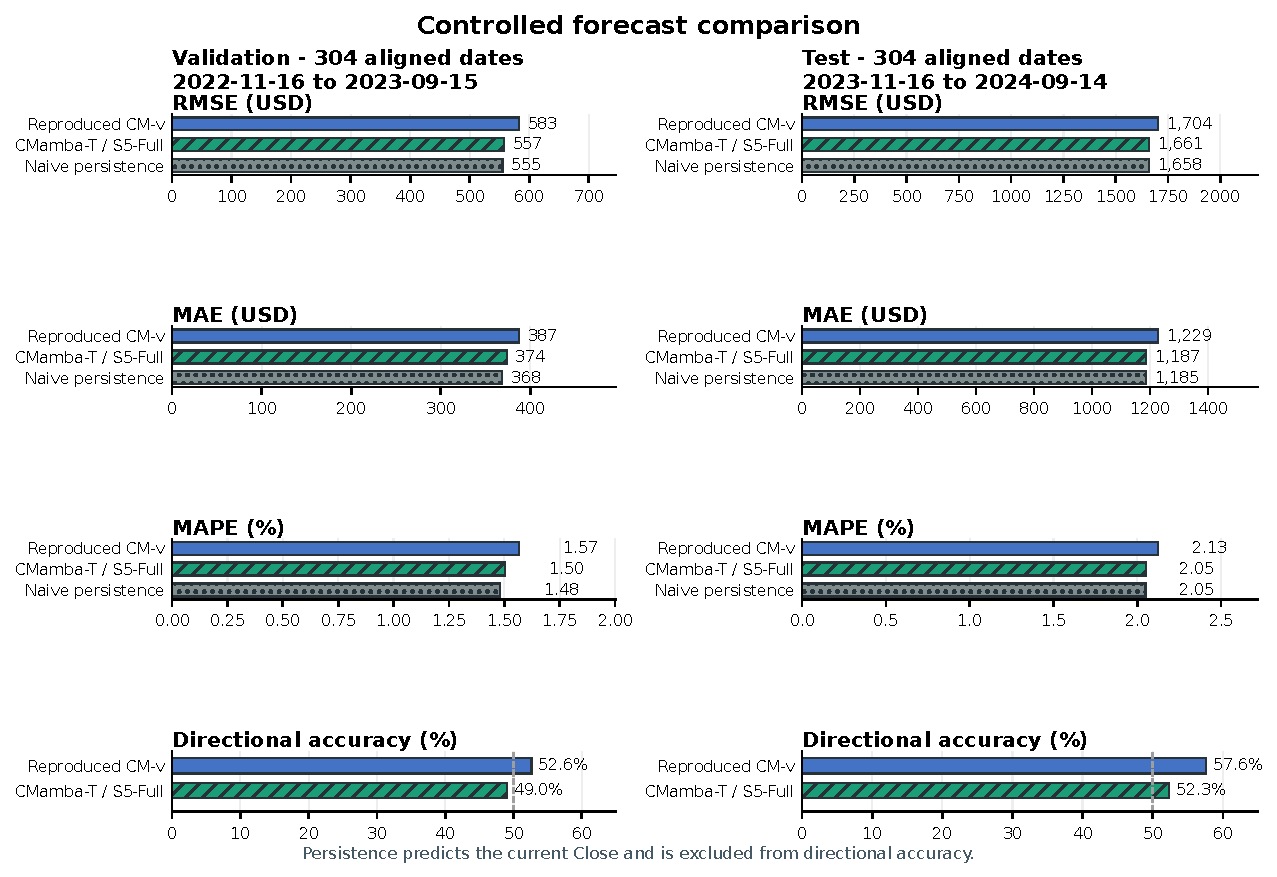
\includegraphics[width=\linewidth]{figures/controlled_forecast.pdf}
\caption[Controlled forecast comparison]{Controlled validation and test comparison on 304 aligned
target dates per split. Directional accuracy is reported only for CM-v and S5-Full.}
\label{fig:controlled-forecast}
\end{figure}

The point estimates show lower error for S5-Full than CM-v on both splits, while persistence remains
lower than S5-Full. CM-v has the highest test directional accuracy. Price-level error and
directional prediction measure different properties and must be interpreted separately.

\begin{table}[H]
\centering
\caption{Moving-block-bootstrap 95\% confidence intervals for RMSE. $\Delta$RMSE is S5-Full minus CM-v.}
\label{tab:rmse-ci}
{\scriptsize
\begin{tabular}{@{}lrrrr@{}}
\toprule
\textbf{Split} & \textbf{CM-v} & \textbf{S5-Full} & \textbf{Persistence} & \textbf{$\Delta$RMSE [95\% CI]} \\
\midrule
Val & [\num{490.30}, \num{684.89}] & [\num{477.58}, \num{644.61}] & [\num{474.90}, \num{642.26}] & \num{-25.18} [\num{-55.69}, \num{6.54}] \\
Test & [\num{1480.46}, \num{1945.62}] & [\num{1420.73}, \num{1918.17}] & [\num{1419.78}, \num{1914.65}] & \num{-42.69} [\num{-114.49}, \num{23.44}] \\
\bottomrule
\end{tabular}}
\end{table}

\begin{table}[H]
\centering
\caption{Sensitivity of paired 95\% intervals to bootstrap block length. Negative
$\Delta$RMSE favors S5-Full; positive $\Delta$Direction favors CM-v.}
\label{tab:block-sensitivity}
{\scriptsize
\begin{tabular}{@{}lrrr@{}}
\toprule
\textbf{Split} & \textbf{$L$} & \textbf{$\Delta$RMSE [95\% CI]} &
\textbf{$\Delta$Direction [95\% CI, pp]} \\
\midrule
Val & \num{5} & [\num{-55.80}, \num{5.95}] & [\num{-3.29}, \num{10.86}] \\
Val & \num{7} & [\num{-55.69}, \num{6.54}] & [\num{-2.96}, \num{10.86}] \\
Val & \num{14} & [\num{-53.02}, \num{4.23}] & [\num{-2.30}, \num{10.20}] \\
\midrule
Test & \num{5} & [\num{-116.46}, \num{23.53}] & [\num{-3.62}, \num{12.83}] \\
Test & \num{7} & [\num{-114.49}, \num{23.44}] & [\num{-3.29}, \num{12.50}] \\
Test & \num{14} & [\num{-106.55}, \num{16.23}] & [\num{-2.63}, \num{11.51}] \\
\bottomrule
\end{tabular}}
\end{table}

Every interval in Table~\ref{tab:block-sensitivity} includes zero. Thus neither paired conclusion
changes for $L=\num{5},\num{7},\num{14}$: no RMSE or directional advantage is statistically
confirmed. This is a bounded sensitivity check over three dependence settings, not a claim for
arbitrary block lengths.

RMSE penalizes error magnitude, whereas directional accuracy compares only the sign of change. On
test, the median absolute predicted return is \num{0.67}\% for CM-v and \num{0.12}\% for S5-Full;
staying closer to the current price can reduce S5-Full's squared error without improving direction.
On validation, the 95\% directional-accuracy intervals are [\num{47.37}, \num{59.21}]\% for CM-v
and [\num{44.41}, \num{54.28}]\% for S5-Full; their difference is \num{3.62} percentage points
with interval [\num{-2.96}, \num{10.86}]. On test, the corresponding intervals are
[\num{51.32}, \num{62.83}]\%, [\num{47.70}, \num{57.24}]\%, and a \num{5.26}-point difference
with interval [\num{-3.29}, \num{12.50}]. Both paired intervals include zero. Exact McNemar tests
did not reject the null of equal marginal directional accuracy (validation $p=\num{0.400}$; test
$p=\num{0.224}$); this is not evidence of equivalence.

\begin{table}[H]
\centering
\caption{Descriptive chronological-half comparison; each period contains 152 consecutive dates.}
\label{tab:temporal-stability}
{\scriptsize
\begin{tabular}{@{}lrrrrr@{}}
\toprule
\textbf{Period} & \textbf{CM-v RMSE} & \textbf{S5 RMSE} & \textbf{Persistence RMSE} & \textbf{CM-v Dir. (\%)} & \textbf{S5 Dir. (\%)} \\
\midrule
Val H1 & \num{599.05} & \num{561.60} & \num{559.57} & \num{50.66} & \num{48.68} \\
Val H2 & \num{565.49} & \num{553.04} & \num{550.27} & \num{54.61} & \num{49.34} \\
Test H1 & \num{1693.50} & \num{1669.26} & \num{1672.69} & \num{59.21} & \num{53.29} \\
Test H2 & \num{1713.47} & \num{1652.35} & \num{1642.26} & \num{55.92} & \num{51.32} \\
\bottomrule
\end{tabular}}
\end{table}

Val H1/H2 cover 16-11-2022--16-04-2023 and 17-04-2023--15-09-2023; Test H1/H2 cover
16-11-2023--15-04-2024 and 16-04-2024--14-09-2024. S5-Full has lower RMSE than CM-v in all four
periods, but persistence is lower than S5-Full in three; CM-v has higher directional accuracy in all
four. This is a descriptive check on the same checkpoints, not four training runs or four independent
holdouts.

\begin{table}[H]
\centering
\caption{Paired tests on 304 common dates. DM uses squared error with HAC lag 1; Wilcoxon uses
absolute error.}
\label{tab:paired-tests}
{\small
\begin{tabularx}{\linewidth}{@{}llrrll@{}}
\toprule
\textbf{Split} & \textbf{Comparison A vs B} & \textbf{DM $p$} & \textbf{Wilcoxon $p$} & \textbf{Lower MSE} & \textbf{Lower MAE} \\
\midrule
Val & CM-v vs persistence & \num{0.106} & \textbf{\num{0.024}} & persistence & persistence \\
Val & S5-Full vs persistence & \num{0.161} & \textbf{\num{0.017}} & persistence & persistence \\
Val & S5-Full vs CM-v & \num{0.128} & \num{0.094} & S5-Full & S5-Full \\
\midrule
Test & CM-v vs persistence & \num{0.188} & \num{0.096} & persistence & persistence \\
Test & S5-Full vs persistence & \num{0.455} & \num{0.977} & persistence & persistence \\
Test & S5-Full vs CM-v & \num{0.224} & \num{0.117} & S5-Full & S5-Full \\
\bottomrule
\end{tabularx}}
\end{table}

On validation, Wilcoxon identifies lower absolute error for persistence than for CM-v
($p=\num{0.024}$) and S5-Full ($p=\num{0.017}$); DM does not reject equal squared-error accuracy.
On test, all six $p$-values exceed 0.05. Therefore, S5-Full's lower RMSE than CM-v is an observed
point estimate, not evidence of a statistically significant advantage.

\section{RQ3: Paper Replay and Corrected Self-Financing}\label{sec:rq3-results}
Table~\ref{tab:paper-replay} preserves the paper's zero-cost trading protocol. The official
checkpoint reproduces the three published test rows almost exactly. The reproduced checkpoint
generates a different action sequence, so its ending balance is lower despite only a small
difference in aggregate forecast error.

\begin{table}[htbp]
\centering
\caption{Paper replay on test with \$100 initial capital and zero fees.}
\label{tab:paper-replay}
{\small
\begin{tabularx}{\linewidth}{@{}llrrrr@{}}
\toprule
\textbf{Checkpoint} & \textbf{Strategy} & \textbf{Paper balance} & \textbf{Local balance} & \textbf{Paper MDD (\%)} & \textbf{Local MDD (\%)} \\
\midrule
Official & Vanilla & \num{246.58} & \num{246.58} & \num{23.48} & \num{23.48} \\
Official & Smart & \num{213.20} & \num{213.20} & \num{13.37} & \num{13.37} \\
Official & Extended Smart & \num{262.78} & \num{262.78} & \num{11.09} & \num{11.09} \\
\midrule
Reproduced & Vanilla & \num{246.58} & \num{174.94} & \num{23.48} & \num{23.94} \\
Reproduced & Smart & \num{213.20} & \num{165.25} & \num{13.37} & \num{10.20} \\
Reproduced & Extended Smart & \num{262.78} & \num{204.26} & \num{11.09} & \num{11.74} \\
\bottomrule
\end{tabularx}}
\end{table}

Table~\ref{tab:corrected-trading} is a separate evaluation surface: 304 common dates, a
self-financing engine, and a 0.2\% fee. Its balances should not be compared directly with
Table~\ref{tab:paper-replay} because the date sets and accounting rules differ.

\begin{table}[htbp]
\centering
\caption{Corrected self-financing test results with a 0.2\% fee and \$100 initial capital. Turnover
and fees are in USD; every reconciliation error is zero.}
\label{tab:corrected-trading}
{\scriptsize
\begin{tabularx}{\linewidth}{@{}Xlrrrrrr@{}}
\toprule
\textbf{Model} & \textbf{Strategy} & \textbf{Final} & \textbf{ROI (\%)} & \textbf{MDD (\%)} & \textbf{Trades} & \textbf{Turnover} & \textbf{Fees} \\
\midrule
Shared control & Buy-and-hold & \textbf{\num{158.09}} & \textbf{\num{58.09}} & \num{26.18} & \num{1} & \num{99.80} & \num{0.20} \\
\midrule
Reproduced CM-v & Vanilla & \num{115.97} & \num{15.97} & \num{26.29} & \num{46} & \num{5731.07} & \num{11.46} \\
Reproduced CM-v & Smart & \num{95.92} & \num{-4.08} & \num{18.08} & \num{222} & \num{7758.47} & \num{15.52} \\
Reproduced CM-v & Extended Smart & \num{92.11} & \num{-7.89} & \num{19.81} & \num{304} & \num{19450.28} & \num{38.90} \\
\midrule
S5-Full & Vanilla & \num{100.00} & \num{0.00} & \num{0.00} & \num{0} & \num{0.00} & \num{0.00} \\
S5-Full & Smart & \num{103.08} & \num{3.08} & \num{1.91} & \num{133} & \num{124.35} & \num{0.25} \\
S5-Full & Extended Smart & \num{98.39} & \num{-1.61} & \num{5.00} & \num{304} & \num{508.33} & \num{1.02} \\
\midrule
Persistence & All three modes & \num{100.00} & \num{0.00} & \num{0.00} & \num{0} & \num{0.00} & \num{0.00} \\
\bottomrule
\end{tabularx}}
\end{table}

\begin{figure}[htbp]
\centering
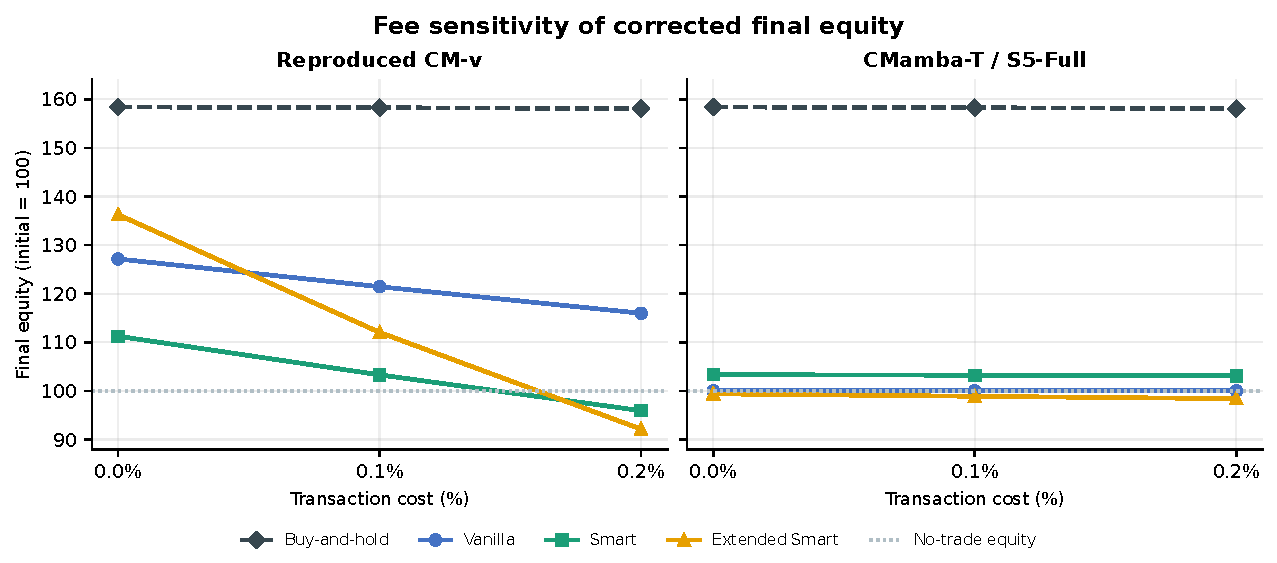
\includegraphics[width=\linewidth]{figures/corrected_trading.pdf}
\caption[Fee sensitivity of corrected final equity]{Fee sensitivity of corrected final equity on
the 304-date test split. Each panel compares Buy-and-hold, Vanilla, Smart, and Extended Smart at
0\%, 0.1\%, and 0.2\% transaction cost.}
\label{fig:corrected-trading}
\end{figure}

No forecast-driven strategy outperforms buy-and-hold at any fee. As cost rises from 0\% to 0.2\%,
CM-v Vanilla falls from \num{127.14} to \num{115.97}, Smart from \num{111.23} to \num{95.92}, and
Extended Smart from \num{136.25} to \num{92.11}. S5-Full Smart changes only from \num{103.34} to
\num{103.08}; Vanilla issues no trades. RQ3 therefore does not depend on choosing 0.2\% alone:
paper replay reproduces the released algorithm, while the corrected engine does not confirm an
economic advantage, and high-turnover policies are more fee-sensitive.

% ---------------------------------------------------------------------
\chapter{CMamba-T/S5-Full Experiment}\label{chap:s5}

\section{Design and Scale}\label{sec:s5-design}
Both official and reproduced CM-v retain the paper's $[B,6,14]$ tensor. In a separate local
experiment, S5-Full receives a sequence of 60 day-tokens with a 32-dimensional embedding. Window
length and model width become independent quantities, a structural difference verifiable in the
source. Because the experiment changes the input window, preprocessing, output parameterization,
and architecture together, it is not an architecture-only ablation.

S5-Full has \num{57249} parameters, or \num{41.80}\% of CM-v, a reduction of \num{58.20}\%.
Figure~\ref{fig:params-error} places this scale beside RMSE on the same splits. Persistence is a
zero-parameter reference line, not a learned-model point.

\begin{figure}[htbp]
\centering
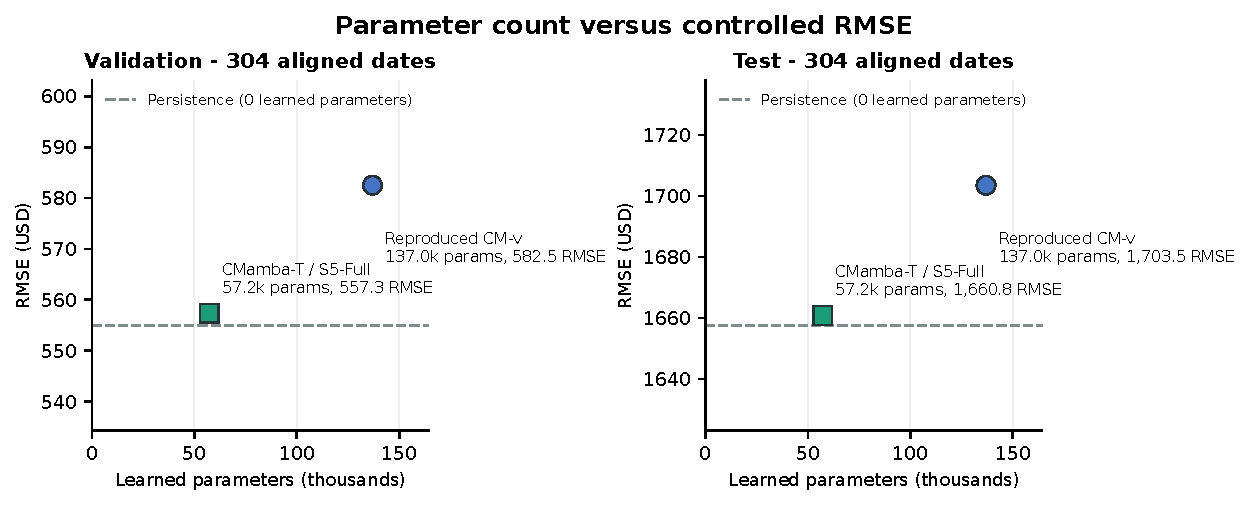
\includegraphics[width=\linewidth]{figures/params_vs_error.pdf}
\caption[Parameter count versus forecast error]{Parameter count versus validation and test RMSE.
Only CM-v and S5-Full are learned models; persistence is a zero-parameter reference.}
\label{fig:params-error}
\end{figure}

\section{Forecasting and Trading Results}\label{sec:s5-results}
S5-Full's RMSE is \num{25.18} below CM-v on validation (\num{557.34} versus \num{582.52}) and
\num{42.69} below on test (\num{1660.83} versus \num{1703.51}), while remaining \num{2.40} and
\num{3.28} above persistence, respectively. Neither S5-Full--CM-v difference is significant under
DM or Wilcoxon (Table~\ref{tab:paired-tests}).

In corrected trading, S5-Full Smart ends between \$\num{103.34} and \$\num{103.08} as cost rises
from 0\% to 0.2\%; Vanilla issues no trades, and Extended Smart ends at \$\num{98.39} at 0.2\%.
Lower forecast error than CM-v therefore does not imply higher profit under every policy.

\section{RQ4 Conclusion}\label{sec:s5-conclusion}
\enlargethispage{2\baselineskip}
S5-Full has lower point-estimate RMSE than reproduced CM-v on validation and test, but not than
persistence. Paired tests and intervals do not establish general superiority. Only the seed-23
checkpoint was evaluated. Forecasts, statistical tests, parameters, and trading characterize this
run, not variation across training runs.

% ---------------------------------------------------------------------
\chapter{Explanatory System}\label{chap:system}

\section{Architecture and Primary Workflow}\label{sec:system-flow}
The system comprises a React/TypeScript frontend, a FastAPI backend, and a Python worker from the
core repository. The backend serves evaluation tables and delegates forecast requests to the worker
that runs the selected checkpoint. Invalid data or an unavailable checkpoint produces an explicit
error instead of a simulated result.

\begin{figure}[htbp]
\centering
\resizebox{\linewidth}{!}{% Primary prediction path with separate analysis and presentation outputs.
\begingroup
\definecolor{flowBlue}{HTML}{E8F0FB}
\definecolor{flowBlueEdge}{HTML}{5A7FBE}
\definecolor{flowGreen}{HTML}{E4F3EC}
\definecolor{flowGreenEdge}{HTML}{418B72}
\definecolor{flowGold}{HTML}{FFF1CF}
\definecolor{flowGoldEdge}{HTML}{B4882C}
\definecolor{flowViolet}{HTML}{F0EAF8}
\definecolor{flowVioletEdge}{HTML}{8068A6}
\definecolor{flowGrey}{HTML}{F5F7F9}
\definecolor{flowGreyEdge}{HTML}{AAB4BD}
\definecolor{flowInk}{HTML}{263238}

\tikzset{
  input/.style={draw=flowBlueEdge, fill=flowBlue, rounded corners=3pt,
    minimum width=1.9cm, minimum height=1.05cm, align=center, inner sep=4pt,
    font=\sffamily\small\bfseries, text=flowInk},
  process/.style={draw=flowGreenEdge, fill=flowGreen, rounded corners=3pt,
    minimum width=2.25cm, minimum height=1.05cm, align=center, inner sep=4pt,
    font=\sffamily\small\bfseries, text=flowInk},
  repeat/.style={draw=flowVioletEdge, fill=flowViolet, rounded corners=3pt,
    minimum width=2.25cm, minimum height=1.05cm, align=center, inner sep=4pt,
    font=\sffamily\small\bfseries, text=flowInk},
  head/.style={draw=flowGoldEdge, fill=flowGold, rounded corners=3pt,
    minimum width=2.25cm, minimum height=1.05cm, align=center, inner sep=4pt,
    font=\sffamily\small\bfseries, text=flowInk},
  output/.style={draw=flowBlueEdge, fill=flowBlue, rounded corners=3pt,
    minimum width=2.1cm, minimum height=1.05cm, align=center, inner sep=4pt,
    font=\sffamily\small\bfseries, text=flowInk},
  group/.style={draw=flowGreyEdge, fill=flowGrey, dashed, rounded corners=6pt,
    line width=0.75pt, inner xsep=7pt, inner ysep=8pt},
  note/.style={font=\sffamily\small\bfseries, text=flowInk, align=left},
  flow/.style={-{Stealth[scale=1.2]}, draw=flowInk, line width=0.85pt},
  junction/.style={circle, draw=flowInk, fill=flowInk, minimum size=3.2pt,
    inner sep=0pt}
}

\begin{tikzpicture}[font=\sffamily\small, node distance=0.6cm and 0.8cm]
  \node[input] (data)
    {OHLCV\\data\\{\scriptsize\mdseries CSV / paper split}};
  \node[process, right=of data] (validate)
    {Validate and\\preprocess\\{\scriptsize\mdseries schema + causal order}};
  \node[process, right=of validate] (select)
    {Select model/\\window\\{\scriptsize\mdseries CM-v: 14; S5-Full: 60}};
  \node[head, right=of select] (inference)
    {Local checkpoint\\inference};
  \node[output, right=of inference] (forecast)
    {Next-day\\forecast};

  \node[note, above=0.34cm of data.north west, anchor=south west] (predictionTitle)
    {Prediction workflow};

  \draw[flow] (data) -- (validate);
  \draw[flow] (validate) -- (select);
  \draw[flow] (select) -- (inference);
  \draw[flow] (inference) -- (forecast);

  \node[junction, below=1.70cm of inference] (analysisHub) {};
  \node[repeat, below=0.65cm of analysisHub] (replay)
    {Historical\\replay\\{\scriptsize\mdseries paper protocol}};
  \node[repeat, left=of replay] (evaluation)
    {Forecast\\evaluation\\{\scriptsize\mdseries common dates + paired tests}};
  \node[repeat, right=of replay] (trading)
    {Corrected\\trading\\{\scriptsize\mdseries self-financing + costs}};
  \node[output, below=of replay] (console)
    {Five-screen\\Console};

  \node[note, above=0.24cm of analysisHub] (analysisTitle)
    {Analysis and presentation};

  \draw[flow] (forecast.south) |- (analysisHub.east);
  \draw[flow] (analysisHub) -- (evaluation.north);
  \draw[flow] (analysisHub) -- (replay.north);
  \draw[flow] (analysisHub) -- (trading.north);
  \draw[flow] (evaluation.south) |- (console.west);
  \draw[flow] (replay) -- (console);
  \draw[flow] (trading.south) |- (console.east);

  \begin{scope}[on background layer]
    \node[group, fit=(predictionTitle)(data)(validate)(select)(inference)(forecast)] {};
    \node[group,
      fit=(analysisTitle)(analysisHub)(evaluation)(replay)(trading)(console)] {};
  \end{scope}
\end{tikzpicture}
\endgroup
}
\caption[System workflow]{Primary workflow from OHLCV validation and local checkpoint inference to
forecast evaluation, historical replay, corrected trading, and the five-screen Console.}
\label{fig:system-flow}
\end{figure}

The primary flow is uploaded or paper data $\to$ CM-v or S5-Full selection $\to$
\emph{local checkpoint} execution $\to$ forecast, expected return, and input window.
CM-v requires at least 14 candles; S5-Full requires 60. Historical replay is an independent mode.
Live HTTP appears under advanced options and sends a request only when explicitly invoked.

\section{Five Screens}\label{sec:five-screens}
The Console retains the five-screen structure, and both the interface and embedded screenshots are
in English. Table~\ref{tab:screens} maps each screen to its thesis role.

\begin{table}[htbp]
\centering
\caption{Roles of the five Console screens.}
\label{tab:screens}
\begin{tabularx}{\linewidth}{@{}lXX@{}}
\toprule
\textbf{Screen} & \textbf{Function} & \textbf{Displayed result} \\
\midrule
Data & Load CSV; validate schema, order, values, and history & Validated OHLCV \\
Evaluation & Compare reported values, local metrics, and paired tests & Forecast metrics \\
Predict & Select checkpoint; forecast paper or new data; separate replay & Next-day price \\
Trading & Switch between paper replay and corrected self-financing & Two trading protocols \\
Architecture & Compare the paper description, released CM-v path, and S5-Full & Model architecture \\
\bottomrule
\end{tabularx}
\end{table}

\begin{figure}[p]
\centering
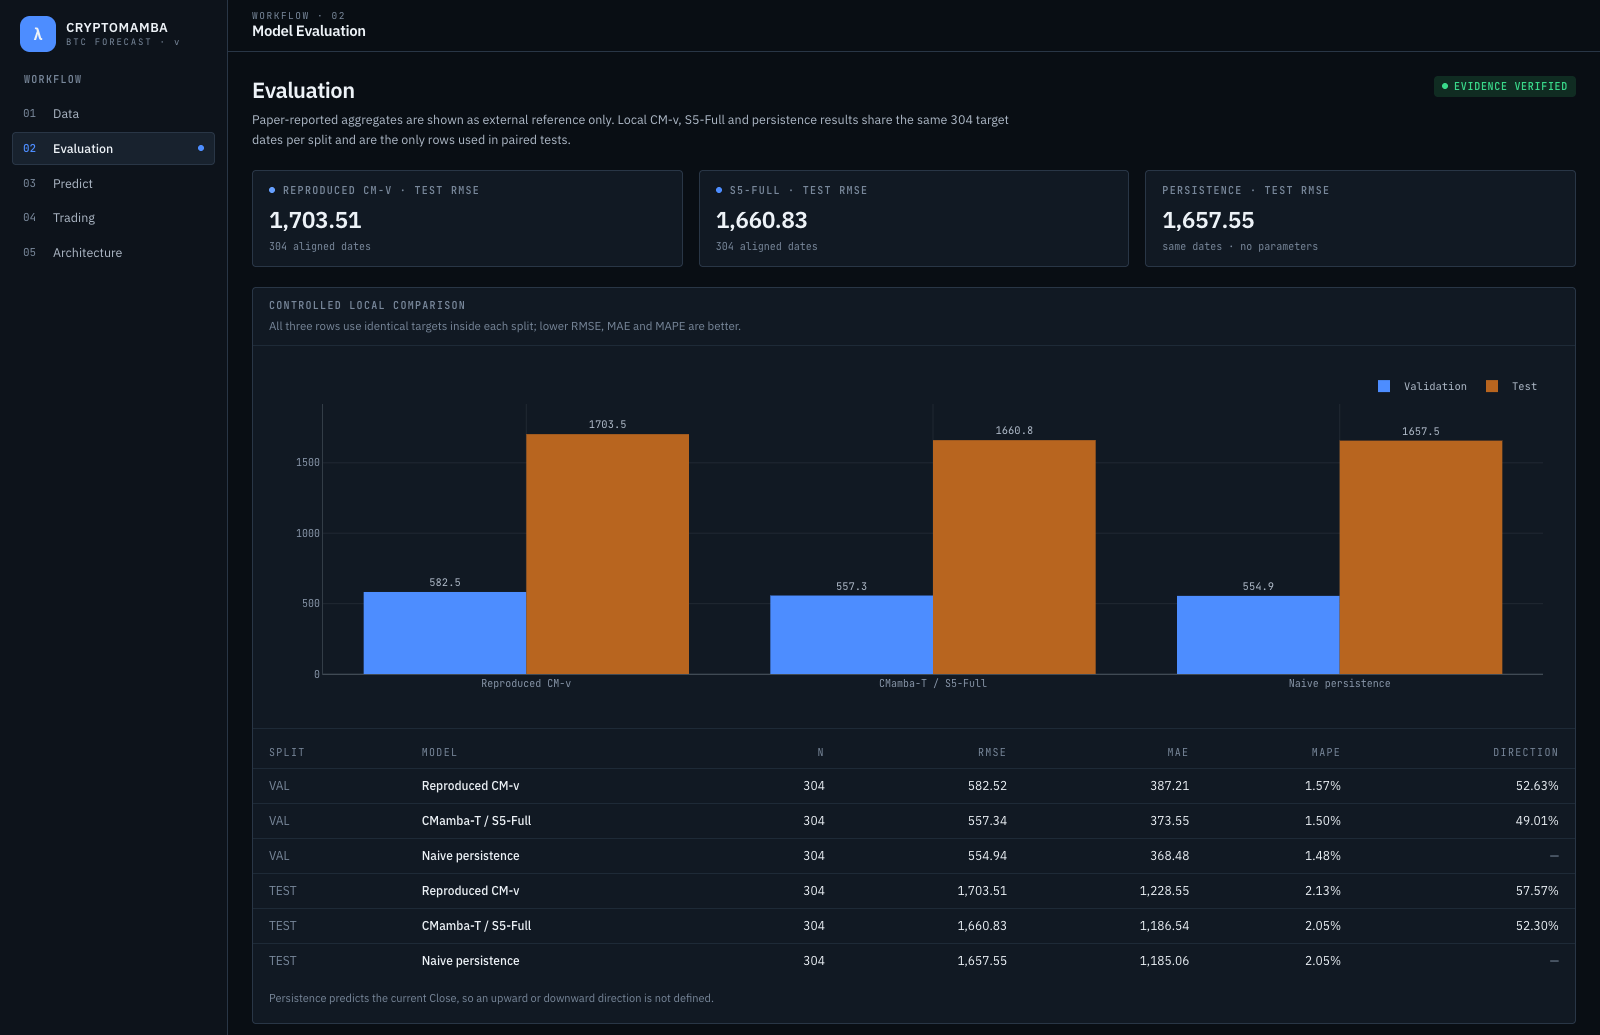
\includegraphics[width=\linewidth]{figures/ui/ui_evaluation.png}
\caption[Evaluation screen]{Evaluation screen: controlled validation/test RMSE and the aligned
local metric table.}
\label{fig:ui-evaluation}
\end{figure}

\begin{figure}[p]
\centering
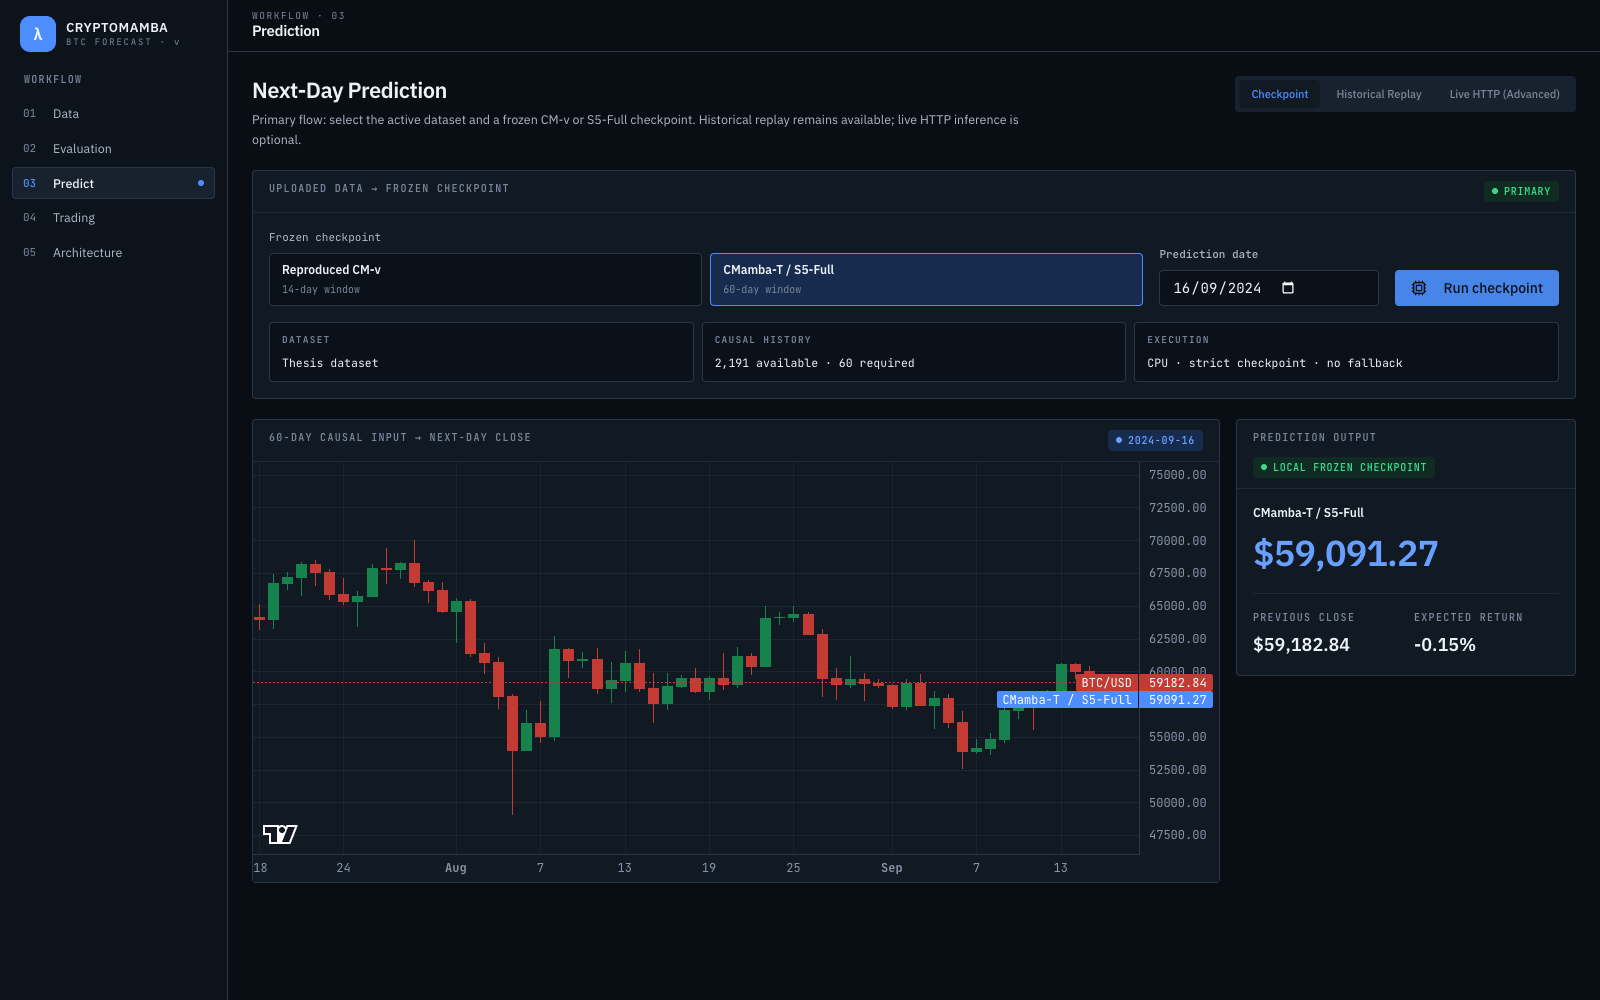
\includegraphics[width=\linewidth]{figures/ui/ui_predict.png}
\caption[Predict screen]{Predict screen: uploaded or paper data is sent to the selected CM-v or
S5-Full local checkpoint; the model window remains visible.}
\label{fig:ui-predict}
\end{figure}

\begin{figure}[p]
\centering
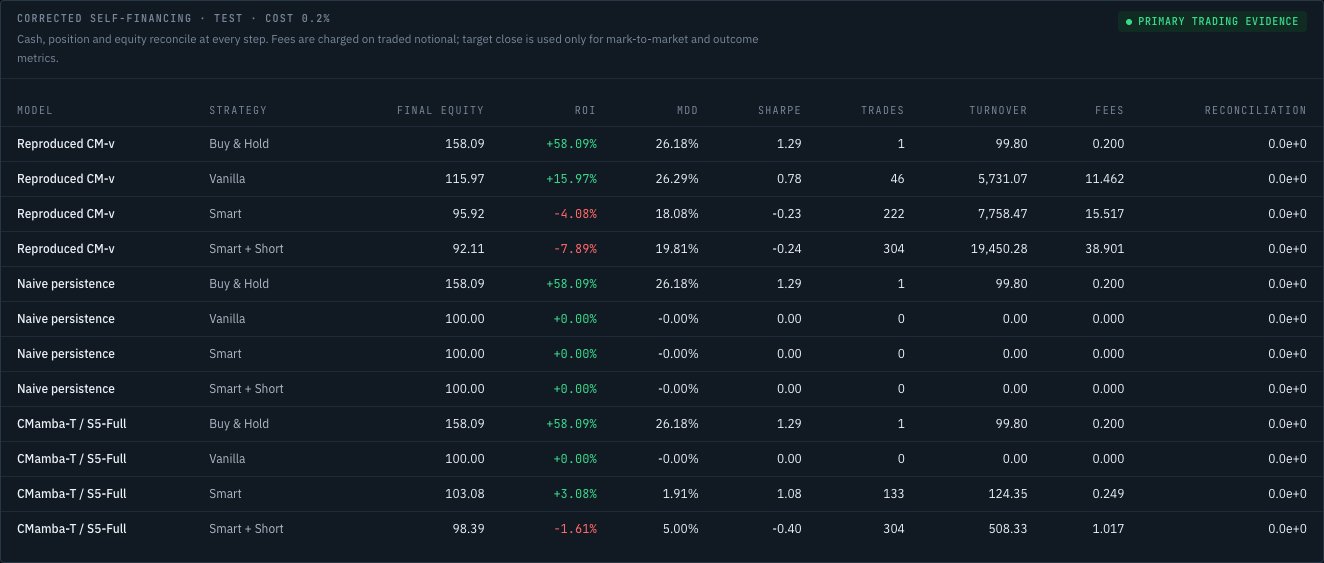
\includegraphics[width=\linewidth]{figures/ui/ui_trading.png}
\caption[Trading screen]{Trading screen: the corrected self-financing result is shown separately
from the original paper replay.}
\label{fig:ui-trading}
\end{figure}

\section{Functional Validation}\label{sec:system-validation}
Automated tests cover CSV parsing, window limits, both model-inference paths, invalid data, and
accounting invariants. Browser checks cover all five screens, both checkpoints, valid and invalid
CSV files, fewer than 60 days of history, historical replay, and both trading protocols. These
checks establish prototype functionality; the thesis makes no usability claim without a user study.

% ---------------------------------------------------------------------
\chapter{Discussion and Conclusion}\label{chap:discussion}

\section{Answers to the Research Questions}\label{sec:answers}
\textbf{RQ1.} The official checkpoint reproduces the forecasts and paper trading replay almost
exactly. On the 350-day protocol, the reproduced checkpoint differs from the reported result by
\num{0.892}\% RMSE, \num{1.057}\% MAE, and \num{0.718}\% MAPE.

\textbf{RQ2.} On the 304 common target dates in each split, persistence has the lowest RMSE on
both validation and test. S5-Full has lower RMSE than CM-v in all four chronological halves, but
the paired bootstrap intervals include zero and DM does not confirm a difference. CM-v has higher
directional accuracy, but neither the paired interval nor McNemar's test confirms an advantage.
These conclusions are unchanged for bootstrap block lengths \num{5}, \num{7}, and \num{14}.
Price-level error and direction measure different properties.

\textbf{RQ3.} Paper replay confirms reproduction of the released algorithms. With the
self-financing engine, no forecast-driven strategy outperforms buy-and-hold at 0\%, 0.1\%, or 0.2\%
cost on the same 304 test dates. Turnover explains the fee sensitivity of frequently trading
policies.

\textbf{RQ4.} S5-Full reduces parameter count by \num{58.20}\% and has lower RMSE than CM-v on both
measured splits, but does not outperform persistence. Its model contribution is therefore a
lightweight experiment evaluated across forecasting, statistical testing, and trading, not a claim
of the best model.

\section{Limitations}\label{sec:limitations}
\begin{itemize}
\item The data cover one asset, one frequency, and one horizon. Rankings do not automatically
generalize to other assets or periods.
\item The 60-day S5-Full window was not compared with alternatives. The historical test set has
already been used for reporting, so subsequent decisions require a new holdout.
\item The corrected engine retains signal-day Close execution for reconciliation. This same-close
abstraction must be replaced by next-open execution with observed slippage, spread, and borrow
costs for a realistic evaluation.
\item The Console is a local prototype. It has not undergone load testing, deployment security
audit, user research, or integration with an order-management system.
\end{itemize}

\section{Future Work}\label{sec:future}
The first priority is to freeze the current protocol and evaluate it once on a holdout after
09-2024, followed by multiple S5-Full seeds and window comparison under a fixed validation
protocol. Later extensions may add exogenous data, multiple assets, and additional horizons. The
trading engine should adopt next-open execution with a
complete cost model. Live HTTP may be added as an optional adapter after operational validation; it
does not change the local-checkpoint contract.

\newpage
\section{Conclusion}\label{sec:conclusion}
This thesis does more than repeat a published result table. It separates Paper-reported values from
local results, aligns every comparison on common dates, adds persistence and paired tests,
reconciles paper replay, and implements a corrected self-financing backtest. S5-Full extends the work
from reproduction to a lightweight model experiment, while its conclusions remain bounded by
persistence and statistical significance. The five-screen Console presents the complete
data--prediction--evaluation--trading--architecture chain directly from local checkpoints.

Within Vietnam's pilot crypto-asset market, the prototype's application value lies in result
visualization and explicit experimental limitations, not in issuing investment signals.

% ---------------------------------------------------------------------
\section*{Data and Code Availability}\label{sec:availability}
\addcontentsline{toc}{section}{Data and Code Availability}

The original paper and source code are available at \url{https://arxiv.org/abs/2501.01010} and
\url{https://github.com/MShahabSepehri/CryptoMamba}. The forecast, statistical, and trading data used
in the result tables are supplied with the project materials.

% ---------------------------------------------------------------------
\begin{thebibliography}{99}
\addcontentsline{toc}{chapter}{References}

\bibitem{cryptomamba}
Sepehri, M. S., Mehradfar, A., Soltanolkotabi, M., and Avestimehr, S.
\textit{CryptoMamba: Leveraging State Space Models for Accurate Bitcoin Price Prediction}.
IEEE ICBC, 2025; arXiv:2501.01010v2. \url{https://arxiv.org/abs/2501.01010}.

\bibitem{mamba}
Gu, A. and Dao, T. \textit{Mamba: Linear-Time Sequence Modeling with Selective State Spaces}.
arXiv:2312.00752, 2023. \url{https://arxiv.org/abs/2312.00752}.

\bibitem{itransformer}
Liu, Y. et al. \textit{iTransformer: Inverted Transformers Are Effective for Time Series
Forecasting}. ICLR, 2024. \url{https://openreview.net/forum?id=JePfAI8fah}.

\bibitem{smamba}
Wang, Z. et al. \textit{Is Mamba Effective for Time Series Forecasting?}
arXiv:2403.11144, 2024. \url{https://arxiv.org/abs/2403.11144}.

\bibitem{dm}
Diebold, F. X. and Mariano, R. S. \textit{Comparing Predictive Accuracy}.
Journal of Business \& Economic Statistics, 13(3), 253--263, 1995.
\url{https://doi.org/10.1080/07350015.1995.10524599}.

\bibitem{wilcoxon}
Wilcoxon, F. \textit{Individual Comparisons by Ranking Methods}.
Biometrics Bulletin, 1(6), 80--83, 1945. \url{https://doi.org/10.2307/3001968}.

\bibitem{neweywest}
Newey, W. K. and West, K. D. \textit{A Simple, Positive Semi-Definite, Heteroskedasticity and
Autocorrelation Consistent Covariance Matrix}. Econometrica, 55(3), 703--708, 1987.
\url{https://doi.org/10.2307/1913610}.

\bibitem{kunsch1989}
Künsch, H. R. \textit{The Jackknife and the Bootstrap for General Stationary Observations}.
The Annals of Statistics, 17(3), 1217--1241, 1989.
\url{https://doi.org/10.1214/aos/1176347265}.

\bibitem{buhlmann1999}
Bühlmann, P. and Künsch, H. R. \textit{Block Length Selection in the Bootstrap for Time Series}.
Computational Statistics \& Data Analysis, 31(3), 295--310, 1999.
\url{https://doi.org/10.1016/S0167-9473(99)00014-6}.

\bibitem{mcnemar1947}
McNemar, Q. \textit{Note on the Sampling Error of the Difference between Correlated Proportions or
Percentages}. Psychometrika, 12(2), 153--157, 1947.
\url{https://doi.org/10.1007/BF02295996}.

\bibitem{nq05}
Government of the Socialist Republic of Vietnam. \textit{Resolution No. 05/2025/NQ-CP dated
09-09-2025 on the Pilot Crypto-Asset Market in Vietnam}. 2025.
\url{https://vanban.chinhphu.vn/?pageid=27160&docid=215249}.
\end{thebibliography}

\end{document}
